\section{Temperature sensor (Analog)}
\begin{figure}[H]
    \centering
    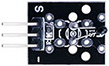
\includegraphics[angle=0, keepaspectratio=true, scale=1, width=200px, height=200px]{images/temperature_analog.jpg}
    %\caption{Caption}
\end{figure}
\subsection*{Description}
A temperature sensor uses a thermistor (a resistor that changes resistance with temperature) and is used to measure the ambient temperature around the module.
\subsection*{Pin mapping}
This pin mapping corresponds to the pins from left to right with the module pins facing towards you.
\begin{table}[H]
    \centering
    \begin{tabular}{|c|c|c|c|c|}
    \hline
    Index &Label &Type &Name &Description\\ \hline
    0 &S &Digital input &D0 &Signal to turn on module\\ \hline
    1 & &Source voltage &$V+$ &Unused\\ \hline
    2 &- &Ground &GND &\\ \hline
    \end{tabular}
    %\caption{Caption}
    %\label{tab:my_label}
\end{table}
\subsection*{Operation}
The output voltage at the analog pin (A0) is related to the ambient temperature around the sensor. Calculating the temperature from the output reading requires some work so refer to the listing associated with this module.
%\subsection*{Code}
%\lstinputlisting[caption=test]{laser.py}